本项目团队致力于开发一个综合性的医疗预约管理系统,该系统以事件为中心,旨在为患者提供全面而便捷的医疗服务体验。系统架构采用了经典的三层结构设计,包括表示层、业务逻辑层和数据访问层,每一层都承载特定的功能和责任,确保了系统的清晰性和可维护性。

在进行系统架构设计时,我们考虑了多种体系结构风格,并最终确定了最适合我们项目需求的架构。以下是我们参考的体系结构风格及其特点:

- \textbf{以数据为中心的体系结构}:这种风格专注于数据的组织和管理,适用于数据存储和处理至关重要的系统。它包括数据存储、数据访问层、业务逻辑层和表示层。

- \textbf{数据流体系结构}:专注于数据的移动和转换,通过一系列处理步骤的数据流来组织系统,适用于需要实时处理或分析的系统。

- \textbf{调用和返回体系结构}:也称为面向过程的架构,通过函数调用和返回进行通信,适用于过程编程语言。

- \textbf{面向对象体系结构}:围绕对象组织系统,对象是封装数据和行为的类的实例,适用于面向对象的编程语言。

- \textbf{分层次体系结构}:将系统组织成层,每一层为其上层提供服务并使用其下层的服务,适用于企业和Web应用程序。

- \textbf{客户端-服务器架构}:将系统分为处理用户界面的客户端和处理业务逻辑的服务器端,适用于网络应用程序。

- \textbf{浏览器-服务器架构}:一种特殊的客户端-服务器架构,客户端运行在用户Web浏览器中,适用于Web应用程序。

- \textbf{微服务架构}:将应用程序构建为小型独立服务的集合,每个服务都专注于特定的业务功能,适用于需要高度可扩展性和灵活性的系统。

- \textbf{事件驱动架构}:强调系统内发生的事件的产生、检测、消费和反应,适用于需要实时处理的应用程序。

我们的医疗预约管理系统采用了分层次体系结构,其中:

- \textbf{表示层}:负责与用户交互,展示信息和接收输入。

- \textbf{业务逻辑层}:处理用户请求,执行业务规则和逻辑。

- \textbf{数据访问层}:作为系统与数据库之间的桥梁,负责数据的存储和检索。

这种架构风格允许我们实现关注点分离,使得开发、测试和维护更加高效。同时,我们也考虑到了系统的可扩展性和未来的技术发展,确保系统能够适应不断变化的需求。

通过精心设计的架构和功能,我们的医疗预约管理系统将提供一个无缝、高效的医疗服务体验,提高医疗服务的可及性和效率,确保用户享受到高质量的医疗服务。这不仅将提升病人的满意度,也将促进医疗服务的整体改进和发展。

\subsection{以数据为中心的体系结构}

以数据为中心的体系结构是一种基于数据处理和数据存储的 IT 架构。它将数据的收集、处理、存储和使用放在整个系统的核心位置,从而使得数据成为整个系统的主要驱动力。以数据为中心的体系结构是一种将数据处理和存储作为系统核心的设计方法。这种架构风格特别适用于那些以数据密集型操作为主的应用场景,如数据库系统、数据仓库、商业智能和大数据分析等。在这样的系统中,数据的组织、管理和优化是最为关键的考量因素。

在以数据为中心的体系结构中,通常包含以下几个关键组件:

1. \textbf{数据存储}:作为架构的核心,负责所有数据的存储和管理。这通常涉及到关系型或非关系型数据库、文件系统或其他形式的数据存储解决方案。数据存储的设计要确保数据的完整性、安全性和高可用性。

2. \textbf{数据访问层}:提供与数据存储交互的接口。这一层可能包含数据访问对象(DAO)、数据映射器或对象关系映射(ORM)框架等,以简化对数据存储的访问和操作。此外,数据访问层还可能负责处理缓存机制、数据库连接管理和事务控制。

3. \textbf{业务逻辑层}:处理与数据相关的业务规则和逻辑。这一层包含了实现系统功能的服务类、控制器和域对象等。业务逻辑层与数据访问层紧密交互,执行数据的检索、处理和存储。

4. \textbf{表示层}:负责将数据呈现给用户,并处理用户的输入。这可以包括图形用户界面、网页界面或API接口等。表示层与业务逻辑层交互,以展示数据和响应用户操作。

以数据为中心的架构强调了数据模型的设计质量,它可以带来一系列的好处,包括提高数据质量管理、优化系统性能以及简化系统的维护和演进。然而,这种架构也存在一些挑战,比如可能会增加系统的复杂性,并且需要专业的技能和工具来支持数据存储和处理的需求。

在医疗预约管理系统中,采用以数据为中心的体系结构可以确保患者信息、预约记录、医疗资源等关键数据的安全性和准确性。同时,通过精心设计的数据模型和访问层,可以提高系统的查询效率和响应速度,从而提升用户体验。尽管这可能需要更多的前期设计工作和专业技能,但从长远来看,它能够为系统提供一个坚实的数据基础,支持未来的扩展和维护。

\begin{figure}[htbp]
	\centering
	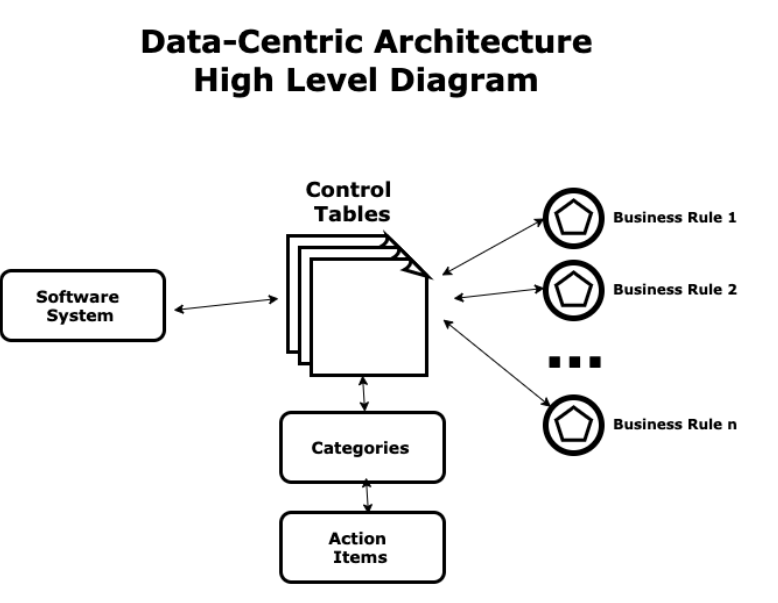
\includegraphics[width=0.6\textwidth]{figures/09.png}
	\caption{以数据为中心的体系结构}
\end{figure}

\subsection{数据流体系结构}
数据流体系结构是一种特别关注于数据在软件系统中流动和转换方式的架构风格。与将系统划分为离散层次或组件的传统方法不同,数据流体系结构通过一系列连续的处理步骤来组织数据的流动。

在数据流体系结构中,以下是几个关键组件:

\textbf{来源(Source)}:这是系统接收初始输入数据的地方。来源可以是传感器、输入设备或其他数据源,负责提供数据流的起点。

\textbf{处理器(Processor)}:处理器对来自来源的数据执行各种处理步骤。这可能包括数据转换、数据清洗、数据聚合或应用机器学习算法等。

\textbf{下沉(Sink)}:下沉组件接收处理器的输出数据,并将其作为最终结果提供给用户或其他下游系统。下沉可以是输出设备、数据库或另一个系统,负责数据流的终止。

连接器(Connector):连接器组件负责在来源、处理器和下沉之间提供通信和协调机制。这可能包括消息队列、事件中心、RESTful API或其他中间件,确保数据能够顺畅地在系统中流动。

数据流体系结构在需要处理大量数据流,尤其是需要实时处理和分析的系统中特别有用。例如,在金融交易、医疗保健监控、物联网设备数据处理等领域,这种架构能够提供高性能、可扩展性和灵活性。

数据流体系结构的优点包括:

1. \textbf{性能改进}:通过优化数据处理步骤,系统可以更高效地处理大量数据。

2. \textbf{可扩展性}:系统可以通过增加处理器或调整数据流来轻松扩展。

3. \textbf{灵活性}:数据流可以根据需要灵活地调整或重新配置。

然而,这种架构也带来了一些挑战:

设计复杂性:设计一个高效的数据流可能非常复杂,需要仔细规划和考虑。
调试难度:由于数据在多个处理步骤中流动,调试和识别问题来源可能比较困难。
专业技能需求:实现和维护数据流体系结构可能需要特定的专业技能和工具。
在医疗预约管理系统中,数据流体系结构可以用来优化患者数据的处理、预约流程的自动化管理以及实时更新医疗资源的状态。通过精心设计的数据流,系统可以实时响应预约变化,提高医疗服务的响应速度和整体效率。

\subsection{调用和返回体系结构}

调用和返回体系结构,亦称为面向过程的架构,是一种传统的软件系统组织方式。在这种架构风格中,系统由一系列的函数或过程组成,这些函数通过彼此之间的调用和返回来实现通信和数据交换。这种架构在早期编程语言中非常普遍,如C语言和Fortran语言,至今仍在某些场景下使用。

面向过程的架构包含以下几个关键组件:

1. \textbf{过程(Procedures)}:这些是系统的构建块,每个过程负责执行一个或一组特定的任务。过程之间可以通过调用来交互,实现任务的委托和数据的传递。

2. \textbf{数据(Data)}:在面向过程的架构中,数据通常以全局变量或局部变量的形式存在,可以在不同的过程间共享。数据通过函数参数传递,或者作为函数的返回值。

3. \textbf{控制流(Control Flow)}:系统的执行流程由函数调用的顺序决定。通常,一个main函数作为程序的入口点,根据程序的需要调用其他函数来完成任务。

面向过程的架构提供了以下优势:

1. 简单性:对于简单的程序,面向过程的架构易于理解和实现。

2. 模块化:程序被分解为模块化的函数,有助于代码的组织。

3. 易于测试和调试:由于程序被分解为独立的函数,测试和调试相对容易。

然而,面向过程的架构也面临一些挑战:

\textbf{抽象有限}:与面向对象的架构相比,面向过程的架构提供的抽象级别较低。
\textbf{代码重复}:由于缺乏类和对象的重用机制,代码重复是一个常见问题。
\textbf{状态管理困难}:在多个过程之间维护和同步状态数据可能会变得复杂。
尽管面向过程的架构在某些特定场合下仍然适用,但它在很多情况下已经被更现代的架构风格所取代,如面向对象的架构和事件驱动的架构。这些现代架构提供了更高级的抽象和功能,更适合管理复杂的系统。

在医疗预约管理系统的背景下,面向过程的架构可能适用于一些简单的数据处理任务,但对于整个系统的开发和维护,可能需要考虑采用更先进的架构风格,以支持系统的可扩展性、灵活性和长期的可维护性。

\subsection{面向对象体系结构}
在软件架构设计中,面向对象体系结构(Object-Oriented Architecture, OOA)是一种以对象为中心的设计风格,它强调了数据和方法的封装、继承和多态性。面向对象的体系结构通常适用于像Java、C++和Python这样的面向对象编程语言,其主要组件包括:

\begin{itemize}
	\item \textbf{类(Class)}:定义了对象的数据结构和行为。类是对象的蓝图,可以通过实例化来创建具体的对象。类之间可以通过继承关系共享数据和行为。
	
	\item \textbf{对象(Object)}:是类的实例,封装了数据和方法。对象之间通过方法调用进行交互,这些方法可以操作对象内部的数据或返回新的数据。
	
	\item \textbf{封装(Encapsulation)}:是一种将对象的实现细节隐藏起来,同时只暴露一个公共接口的做法。封装有助于保护对象的内部状态不被外部直接修改,从而维护系统的完整性和一致性。
	
	\item \textbf{继承(Inheritance)}:允许新类从现有类中继承数据和行为,从而实现代码的重用,并能够创建出具有附加或修改行为的新类。
	
	\item \textbf{多态(Polymorphism)}:允许不同类的对象被视为同一类型的对象,只要它们共享一个公共接口或超类。多态性使得编写的代码能够对不同类型的对象执行相同的操作。
\end{itemize}

面向对象的体系结构提供了模块化、可重用性和可扩展性等显著优势。此外,面向对象的系统通常更易于测试和调试,并能提供对复杂系统的直观表示。

然而,面向对象的体系结构也带来了一些挑战,如管理类层次结构和依赖关系的复杂性,以及维护封装和信息隐藏的难度。

另一方面,分层体系结构(Layered Architecture)是一种将系统组织成多个层次的软件体系结构风格,每一层为其上层提供服务,同时利用其下层的服务。这种风格在企业和Web应用程序中非常常见,其主要组件包括:

\begin{itemize}
	\item \textbf{表示层(Presentation Layer)}:负责向用户展示信息和接收用户输入。这一层可以包括用户界面、网页和应用程序屏幕。
	
	\item \textbf{应用层(Application Layer)}:处理用户输入,并实现系统的业务逻辑。这一层可以包含控制器、管理器和服务类等组件。
	
	\item \textbf{数据层(Data Layer)}:负责数据的存储和检索。这一层可以包括数据访问对象(DAO)、存储库和数据库连接器等组件。
\end{itemize}

每一层通过定义明确的接口或API与其上下层进行通信,上层向下层请求服务,下层通过上层定义的API提供服务。

分层体系结构的优势在于提供了关注点分离、模块化和可扩展性。可以根据需求添加或删除层,以适应不断变化的业务需求,并且每一层都可以独立测试和维护。

然而,分层架构也带来了一些挑战,如管理依赖关系和层间通信的复杂性,以及由于层与层之间的通信开销可能导致的性能问题。分层架构的变体包括n层架构和微服务架构,后者将系统分为小型、独立的服务,这些服务通过API相互通信。

在医疗预约管理系统的背景下,分层体系结构可以清晰地分离表示逻辑、业务逻辑和数据访问逻辑,有助于构建一个可维护、可扩展且易于测试的系统。


\subsection{客户端-服务器架构}
客户端-服务器架构(Client-Server Architecture)是一种常见的软件架构风格,它将系统的功能划分为两个主要部分:客户端和服务器端。这种架构广泛应用于网络应用程序,如Web应用程序、数据库系统和电子邮件系统等。

在客户端-服务器架构中,涉及以下几个关键组件:

\begin{itemize}
	\item \textbf{客户端(Client)}:负责向用户展示信息和处理用户输入。客户端可以是桌面计算机、移动设备或Web浏览器上运行的应用程序。客户端通常负责处理用户界面的呈现和用户的交云操作。
	
	\item \textbf{服务器端(Server)}:负责实现系统的业务逻辑、数据存储和检索。服务器端通常包括用服务器端编程语言(如Java、Python或PHP)编写的代码,以及数据库管理系统(DBMS)。
	
	\item \textbf{通讯层(Communication Layer)}:促进客户端和服务器端之间的通信。这一层通常使用TCP/IP或HTTP(S)等网络协议,包括API、Web服务以及在客户端和服务器端之间交换数据的其他方法。
\end{itemize}

客户端-服务器架构的优势包括:

\begin{itemize}
	\item \textbf{可伸缩性(Scalability)}:服务器端可以轻松扩展以处理增加的流量和用户请求。
	\item \textbf{容错性(Fault Tolerance)}:系统设计可以实现在部分组件失败时继续运行。
	\item \textbf{模块化(Modularity)}:架构的分离性质允许独立的模块开发和维护,便于系统的扩展和维护。
\end{itemize}

然而,客户端-服务器架构也面临一些挑战:

\begin{itemize}
	\item \textbf{安全漏洞(Security Vulnerabilities)}:架构需要妥善处理潜在的安全风险,如数据泄露和恶意攻击。
	\item \textbf{通信复杂性(Communication Complexity)}:管理客户端和服务器端之间的通信可能变得复杂,需要考虑网络延迟和带宽限制。
	\item \textbf{性能问题(Performance Issues)}:网络通信开销可能影响系统性能,特别是在高负载情况下。
	\item \textbf{跨平台一致性(Cross-Platform Consistency)}:由于客户端代码在用户的设备上运行,确保不同设备和平台上的性能和行为一致性是一个挑战。
\end{itemize}

在医疗预约管理系统的背景下,客户端-服务器架构可以提供一个稳定和高效的服务平台,允许用户通过客户端应用程序预约医生、管理个人信息和访问医疗服务。服务器端则集中处理业务逻辑、数据存储和安全性要求。通过精心设计通信层和采用适当的安全措施,可以确保系统的高效运行和数据安全。


\subsection{浏览器-服务器架构}
浏览器-服务器架构(Browser-Server Architecture, BS Architecture),通常称为B/S架构,是一种流行的软件架构模式,特别适用于Web应用程序的开发。在这种架构下,系统被划分为在用户Web浏览器中运行的客户端和在远程服务器上运行的服务器端。

以下是BS架构的主要组件:

\begin{itemize}
	\item \textbf{浏览器(Browser)}:作为客户端,负责向用户展示信息并处理用户输入。浏览器中运行的HTML、CSS和JavaScript代码负责创建用户界面、处理用户交互并将用户请求发送到服务器端。
	
	\item \textbf{服务器端(Server)}:负责实现系统的业务逻辑、数据库的存储和检索操作,并生成动态内容发送回客户端。服务器端通常使用如Java、Python或PHP等服务器端编程语言来实现。
	
	\item \textbf{通讯层(Communication Layer)}:促进客户端和服务器端之间的通信。这一层通常采用HTTP(S)协议,并且可能包括API、Web服务以及客户端和服务器端之间交换数据的其他方法。
\end{itemize}

BS架构的优点包括:

\begin{itemize}
	\item \textbf{灵活性(Flexibility)}:可以在不影响服务器端的情况下更新客户端代码,反之亦然,使得系统维护和升级更加灵活。
	
	\item \textbf{可扩展性(Scalability)}:服务器端可以通过增加硬件资源或优化代码来轻松扩展,以处理更多的用户请求和数据流量。
	
	\item \textbf{易于维护(Maintainability)}:由于客户端和服务器端的分离,使得对任一端的维护和更新都不会影响到另一端。
\end{itemize}

然而,BS架构也存在一些挑战:

\begin{itemize}
	\item \textbf{安全漏洞(Security Vulnerabilities)}:需要特别注意保护系统免受如SQL注入、跨站脚本攻击(XSS)等网络安全威胁。
	
	\item \textbf{通信复杂性(Communication Complexity)}:客户端和服务器端之间的通信可能变得复杂,尤其是在处理大量并发请求时。
	
	\item \textbf{性能问题(Performance Issues)}:网络通信的开销可能影响系统性能,特别是在带宽受限或网络不稳定的情况下。
	
	\item \textbf{跨平台一致性(Cross-Platform Consistency)}:由于客户端代码在用户的设备上运行,确保在不同浏览器和设备上提供一致的用户体验是一个挑战。
\end{itemize}

在医疗预约管理系统的背景下,BS架构可以提供一个用户友好的Web界面,允许患者轻松地预约挂号、查看医疗信息和接收健康咨询。服务器端则集中处理所有后端逻辑和数据存储,确保系统的稳定性和安全性。通过采用BS架构,医疗系统可以实现高效的资源利用和便捷的用户访问,同时降低系统维护和升级的复杂性。

\begin{figure}[htbp]
	\centering
	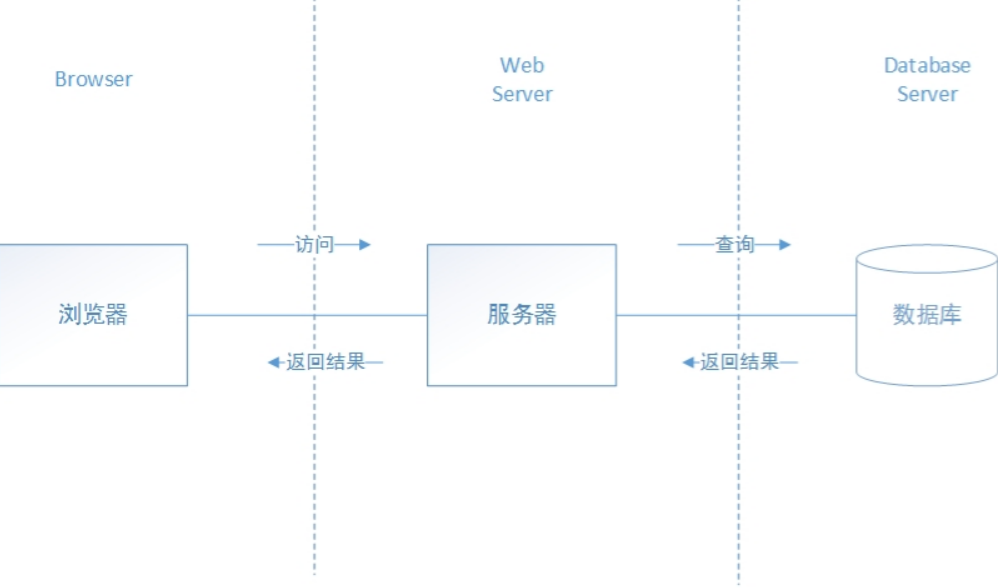
\includegraphics[width=0.6\textwidth]{figures/15.png}
	\caption{B/S体系结构}
\end{figure}


\subsection{微服务架构}
微服务架构(Microservices Architecture)是现代软件开发中一种流行的架构风格,它将一个应用程序构建为一系列小型独立服务的集合,每个服务都专注于实现特定的业务功能。这些服务通过轻量级的通信协议,如HTTP RESTful API或消息队列(例如AMQP或Kafka)进行交互。

微服务架构的关键特征包括:

\begin{itemize}
	\item \textbf{小型独立服务}:每个微服务都是轻量级的,独立运行,并且专注于单一的业务功能。这种设计使得服务易于开发和维护。
	
	\item \textbf{去中心化架构}:在微服务架构中,没有中央控制点,每个服务都可以独立部署、升级和扩展。这种去中心化的特性提高了系统的灵活性和可维护性。
	
	\item \textbf{API通信}:微服务之间通过定义良好的API进行通信,通常采用RESTful接口或轻量级的消息传递协议。这有助于实现服务之间的松耦合。
	
	\item \textbf{领域驱动设计}(DDD):微服务架构通常与领域驱动设计原则结合使用,强调以业务领域为中心进行服务划分和设计。
	
	\item \textbf{开发运营文化}:微服务架构的实施通常伴随着DevOps文化的采纳,即开发和运营团队之间的紧密合作,以及自动化流程和持续交付的实践。
\end{itemize}

微服务架构的优势包括:

\begin{itemize}
	\item \textbf{可扩展性}:可以独立地扩展系统中的单个服务,以应对增加的流量或负载。
	
	\item \textbf{弹性}:由于服务是独立运行的,一个服务的故障不太可能导致整个系统的崩溃。
	
	\item \textbf{灵活性}:团队可以选择最适合其服务的技术栈,并且可以独立地对服务进行更改和迭代。
\end{itemize}

然而,微服务架构也带来了一些挑战:

\begin{itemize}
	\item \textbf{复杂性管理}:随着服务数量的增加,管理和协调这些服务的复杂性也随之增加。
	
	\item \textbf{API通信开销}:服务之间的通信可能涉及额外的网络延迟和开销。
	
	\item \textbf{部署和监控}:需要复杂的工具和流程来部署、监控和维护大量的服务。
	
	\item \textbf{运营成本}:管理多个服务可能会增加运营成本,并且需要更多的DevOps实践来优化流程。
\end{itemize}

在医疗预约管理系统的背景下,微服务架构可以提高系统的可维护性和可扩展性,允许独立地开发和部署各个服务,如用户管理、预约调度、支付处理等。这种架构有助于快速迭代和发布新功能,同时保持系统的高可用性和稳定性。

\subsection{事件驱动架构}
事件驱动架构(Event-Driven Architecture, EDA)是一种软件架构风格,它侧重于系统中事件的生成、检测、消费和响应。这种架构特别适合于需要实时处理的应用程序,如金融交易、传感器网络、电子商务系统等。

在事件驱动架构中,以下是几个关键组件:

\begin{itemize}
	\item \textbf{事件生产者(Event Producers)}:负责生成事件。这些事件可能源自用户操作、传感器读数或系统内部产生的事件。
	
	\item \textbf{事件消费者(Event Consumers)}:负责接收和处理事件。处理通常涉及执行特定的操作,如触发业务逻辑、更新数据库或发送通知。
	
	\item \textbf{事件总线(Event Bus)}:作为事件驱动架构的通信中枢,负责在生产者和消费者之间传递事件。事件总线可以使用如Kafka、RabbitMQ等消息队列系统,或AWS SNS/SQS等云服务来实现。
	
	\item \textbf{事件处理器(Event Processors)}:负责处理事件并执行适当的操作,如数据的聚合、转换或路由到特定的消费者。
\end{itemize}

事件驱动架构的优势包括:

\begin{itemize}
	\item \textbf{可伸缩性(Scalability)}:由于组件的独立性,系统可以根据流量或负载的增加而轻松扩展。
	
	\item \textbf{模块化(Modularity)}:每个组件负责特定的任务,使得系统更加模块化,易于开发和维护。
	
	\item \textbf{容错性(Fault Tolerance)}:组件的独立性还意味着一个组件的故障不太可能影响整个系统的运行。
	
	\item \textbf{技术选择的灵活性(Technological Flexibility)}:团队可以根据需要选择最适合特定组件的技术栈。
\end{itemize}

然而,事件驱动架构也带来了一些挑战:

\begin{itemize}
	\item \textbf{复杂性管理(Complexity Management)}:随着事件生产者和消费者的增加,管理这些组件的复杂性也随之增加。
	
	\item \textbf{事件总线开销(Event Bus Overhead)}:维护事件总线可能需要额外的资源和开销。
	
	\item \textbf{部署和监控(Deployment and Monitoring)}:需要复杂的工具和流程来部署、监控和维护分布式的事件驱动系统。
	
	\item \textbf{调试和排错(Debugging and Troubleshooting)}:异步事件流可能使得系统调试和排错变得更加困难。
\end{itemize}

在医疗预约管理系统中,事件驱动架构可以用于实时处理预约请求、支付确认、医生排班变更等事件。例如,当一个预约被创建或取消时,系统可以实时更新数据库、发送通知给相关方,并触发相关的业务流程。这种架构有助于提高系统的响应速度和可靠性,从而提升患者和医疗机构的整体体验。


\subsection{本次设计采用的体系结构风格}
在本次设计中,评价系统作为医疗预约管理系统的一个重要子模块,是一个基于Web的应用程序。因此,我们采用了多种架构风格的组合来构建这一系统:

\begin{itemize}
	\item \textbf{浏览器-服务器(Browser-Server, B/S)架构}:由于评价系统是一个Web应用程序,它自然地采用了B/S架构。在这种架构中,用户的交互通过Web浏览器进行,而所有的业务逻辑和数据存储都在服务器端处理。
	
	\item \textbf{面向对象体系结构}:系统涉及到用户(包括病人、医生、管理员)和评价等实体,这些实体及其关系是通过对象来表示的。面向对象的方法允许我们通过类和对象来封装数据和行为,提供了一种自然的方式来模拟现实世界中的实体和它们之间的交互。
	
	\item \textbf{事件驱动架构}:评价系统中的许多活动,如添加评价、删除评价等,都可以被视为事件。系统需要检测这些事件并做出相应的响应。事件驱动架构允许系统组件在事件发生时进行通信和交互,从而实现实时响应。
	
	\item \textbf{层次体系结构}:我们的系统采用Spring Boot框架开发,该框架的层次结构从上至下可以分为五层:View层、Controller层、Service层、Mapper层(也称为Dao层)和Model层。每一层都有其特定的职责,且层与层之间通过定义良好的接口进行交互。
	
	\begin{itemize}
		\item \textbf{View层}:负责展示数据给用户,并接收用户输入。
		\item \textbf{Controller层}:负责处理用户的请求,调用Service层的业务逻辑,并准备响应数据。
		\item \textbf{Service层}:包含业务逻辑的应用设计和数据库操作的接口设计。
		\item \textbf{Mapper层}:负责数据持久化,提供CRUD操作。
		\item \textbf{Model层}:存放与数据库表字段相对应的实体类。
	\end{itemize}
	
	\item \textbf{MVC结构}:由于评价系统强调对评价记录等数据的增删改查,并通过中间件与UI界面连接,它也展现了MVC(Model-View-Controller)结构的特点。Model层负责数据,View层负责显示,Controller层负责逻辑。
\end{itemize}

综上所述,本次设计采用的BS体系架构,同时融合了层次体系架构、面向对象体系架构和事件驱动架构的一些特点。这种混合架构风格为评价系统提供了灵活性、可维护性和可扩展性,同时也确保了系统的实时响应能力和用户交互的直观性。通过这种方式,我们的评价系统能够高效地处理用户评价,提升医疗预约管理系统的整体性能和用户体验。



